\chapter{Problem}
An inverted pendulum is to be controlled in an upright position on a moving platform, where the moving platform functions as a disturbance to the system.
% \begin{figure}[htbp]
%         \centering
%         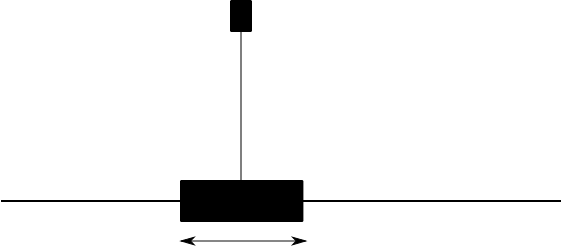
\includegraphics[width=0.6\textwidth,trim=3cm 0cm 3cm 0cm, clip]{pendul.png}
%         \caption{Pendulum on its moving platform}
%         \label{fig:problem}
% \end{figure}
\begin{figure}[H]
        \centering
        \def\svgwidth{10cm}
        \input{figures/pendul.pdf_tex}
        \caption{Shows the inverted pendulum setup with translational disturbance.}
        \label{fig:}
\end{figure}
The model for this system is:
\begin{equation}
        m l \Ddot{\theta} + m g \sin\theta + k_\up{f}  l \ \dot{\theta} = \frac{1}{l}T + \delta_\up{c}(t)
\end{equation}
To simplify the coefficients is parametrised by:
\begin{equation}
        a=\frac{g}{l}, \qquad b=\frac{k_\up{f}}{m}, \qquad c= \frac{k_\up{m}\alpha}{m l^2}, \qquad \delta_\up{c}(t) = k_\up{m} \frac{A\g5}{2000}\sin(t)
\end{equation}

\begin{equation}
        \dot{x}_2 = - a \sin x_1 - b x_2 + c u(t) + \xi(t)
\end{equation}

where
\begin{equation}
        \xi(t) = \frac{1}{m l} \delta_\up{c}(t)
\end{equation}

The system parameters has uncertainties and they are given in the range as follows:
\begin{equation}
        \begin{split}
                l &= 0.305 \, \up{m} \\
                g &= -9.81 \, \frac{\up{m}}{\up{s}^2}\\
                k_\up{m} &= 0.0934 \\
                0.095 \, \text{kg} \leq & m \leq 0.105 \, \text{kg} \\
                0.4 \leq & k_f \leq 0.6 \\
                2/2000 \leq & \alpha \leq 5/2000 \\
                \nonumber
        \end{split}
\end{equation}

The disturbances from the moving platform is roughly:
\begin{equation}
        \delta_c(t) = k_\up{m} \g 5/2000 \g \sin(t)
\end{equation}

The goal is to design a sliding mode controller which can stabilize the inverted pendulum at $(\pi,0)$ with tolerances $|\theta| \leq 0.1$ and $|\dot{\theta}| \leq 0.01$. The controller shall be tested both through simulation and through testing on a real platform.